
%%
%% MIT Thesis - Main Document
%%

\documentclass[12pt]{mitthesis}
\usepackage{lgrind}
\pagestyle{plain}

%\usepackage{thesis}
\usepackage[final]{graphicx}
\usepackage{amsmath,amsfonts,amssymb,amsthm}
\usepackage{verbatim}
\usepackage{color}
\usepackage{floatpag}
\usepackage{float}
\usepackage{listings} %code listing in API section
\lstset{basicstyle= \ttfamily}
\lstset{framesep=4pt}
\lstset{breaklines=true}
\usepackage{multirow}
\usepackage{epsfig}
\usepackage[section]{placeins}
%\usepackage{psfrag}
%\usepackage{makeidx}

%\usepackage[sort]{cite}
%\usepackage{citesort}
\usepackage[numbers,sort&compress,comma]{natbib}

\usepackage[draft=false,letterpaper,breaklinks,colorlinks,linktocpage,citecolor=blue,linkcolor=blue,urlcolor=blue]{hyperref}

% include parts of document
%\includeonly{titlepage,abstract,ack}

%%%%%%%%%%%%%%%%%%%%%%%%%%%%%%%%%%
%% PREAMBLE: Formatting and macros
%%%%%%%%%%%%%%%%%%%%%%%%%%%%%%%%%%

\typeout{}
\typeout{*****************************************************************************}
\typeout{Remember to do the following for LaTeX-ing of final document:}
\typeout{ * spell check .tex and .bib files}
\typeout{ * run BibTex and Index}
\typeout{ * check overfull hboxes}
\typeout{ * check table of contents and, if necessary, ...}
\typeout{ * increment toc page entry of Bibliography and Index}
\typeout{ * comment out the addcontentsline for Bibliography and Index}
\typeout{*****************************************************************************}
\typeout{}

% use footer to denote draft
%\cfoot{\scshape Draft: \today}

% no headers on full-page floats
\floatpagestyle{empty}

% create new float type for algorithm displays
\floatstyle{boxed}
\newfloat{algorithm}{tbh}{loa}
\floatname{algorithm}{Algorithm}
\newcommand{\algtop}{
  \vspace*{-6pt}
  \setlength{\belowdisplayskip}{2pt plus 2pt}
  \setlength{\abovedisplayskip}{2pt plus 2pt}
  \setlength{\itemsep}{4pt}
}
\newcommand{\algend}{
  \vspace*{-2pt}
}

\setlength{\leftmargini}{24pt} \setlength{\leftmarginii}{18pt}

% colors used in some figures
\definecolor{Black}{rgb}{0,0,0}
\definecolor{Blue}{rgb}{0,0,1.0}
\definecolor{Green}{rgb}{0,1.0,0}
\definecolor{Red}{rgb}{1.0,0,0}

\def\shortcite{\cite}

%\makeindex

\begin{document}

%%%%%%%%%%%%%%%
%% Front Matter
%%%%%%%%%%%%%%%

% -*-latex-*-
% $Log: cover.tex,v $
% Revision 1.7  2010/04/29 11:35:46  bryt
% changed department chair from Art Smith to Terry Orlando
% changed default copyright flag from author to MIT, left directions for changing it back
% 
% Revision 1.6  1999/10/21 14:49:31  boojum
% changed comment referring to documentstyle
%
% Revision 1.5  1999/10/21 14:39:04  boojum
% *** empty log message ***
%
% Revision 1.4  1997/04/18  17:54:10  othomas
% added page numbers on abstract and cover, and made 1 abstract
% page the default rather than 2.  (anne hunter tells me this
% is the new institute standard.)
%
% Revision 1.4  1997/04/18  17:54:10  othomas
% added page numbers on abstract and cover, and made 1 abstract
% page the default rather than 2.  (anne hunter tells me this
% is the new institute standard.)
%
% Revision 1.3  93/05/17  17:06:29  starflt
% Added acknowledgements section (suggested by tompalka)
% 
% Revision 1.2  92/04/22  13:13:13  epeisach
% Fixes for 1991 course 6 requirements
% Phrase "and to grant others the right to do so" has been added to 
% permission clause
% Second copy of abstract is not counted as separate pages so numbering works
% out
% 
% Revision 1.1  92/04/22  13:08:20  epeisach
%\pagenumbering{roman}
\thispagestyle{empty}

\title{Spec2Fab: A Reducer-Tuner Model for Translating Specifications to 3D Prints}

\author{Desai Chen}
\prevdegrees{B.S. in Computer Science, Carnegie Mellon University (2011)}
\department{Department of Electrical Engineering and Computer Science}
% If the thesis is for two degrees simultaneously, list them both
% separated by \and like this:
% \degree{Doctor of Philosophy \and Master of Science}
\degree{Master of Science in Computer Science and Engineering}
\degreemonth{September}
\degreeyear{2013}
\thesisdate{Aug 30, 2013}

%% By default, the thesis will be copyrighted to MIT.  If you need to copyright
%% the thesis to yourself, just specify the `vi' documentclass option.  If for
%% some reason you want to exactly specify the copyright notice text, you can
%% use the \copyrightnoticetext command.  
%\copyrightnoticetext{\copyright IBM, 1990.  Do not open till Xmas.}

% If there is more than one supervisor, use the \supervisor command
% once for each.
\supervisor{Wojciech Matusik}{Associate Professor of Electrical Engineering and Computer Science}

% This is the department committee chairman, not the thesis committee
% chairman.  You should replace this with your Department's Committee
% Chairman.
\chairman{Leslie Kolodziejski}{Chairman, Department Committee on Graduate Students}

% Make the titlepage based on the above information.  If you need
% something special and can't use the standard form, you can specify
% the exact text of the titlepage yourself.  Put it in a titlepage
% environment and leave blank lines where you want vertical space.
% The spaces will be adjusted to fill the entire page.  The dotted
% lines for the signatures are made with the \signature command.
\maketitle

% The abstractpage environment sets up everything on the page except
% the text itself.  The title and other header material are put at the
% top of the page, and the supervisors are listed at the bottom.  A
% new page is begun both before and after.  Of course, an abstract may
% be more than one page itself.  If you need more control over the
% format of the page, you can use the abstract environment, which puts
% the word "Abstract" at the beginning and single spaces its text.

%% You can either \input (*not* \include) your abstract file, or you can put
%% the text of the abstract directly between the \begin{abstractpage} and
%% \end{abstractpage} commands.

% First copy: start a new page, and save the page number.
\newpage
% Uncomment the next line if you do NOT want a page number on your
% abstract and acknowledgments pages.
% \pagestyle{empty}

\setcounter{page}{2}
\pagestyle{plain}
\begin{abstractpage}
\chapter*{}
\label{chap:abstract}
\begin{center}
\vspace{-8em}
{\large \textsf{\textbf{Spec2Fab: A Reducer-Tuner Model for Translating Specifications to 3D Prints}}} \\
by (Desai Chen)

\vspace{.2in}

Submitted to the Department of Electrical Engineering and Computer Science \\
in partial fulfillment of the requirements for the degree of \\
Master of Science \\ % <--- replace this with Master of Science if you want a master's instead
\end{center}

\noindent\textsf{\textbf{Abstract}}

\noindent Multi-material 3D printing allows objects to be composed of complex, heterogeneous arrangements of materials. It is often more natural to define a functional goal than to define the material composition of an object. Translating these functional requirements to fabricable 3D prints is still an open research problem. Recently, several specific instances of this problem have been explored (e.g.,  appearance or elastic deformation), but they exist as isolated, monolithic algorithms. In this proposal, I propose an abstraction mechanism that simplifies the design, development, implementation, and reuse of these algorithms. The solution relies on two new data structures: a \emph{reducer tree} that efficiently parameterizes the space of material assignments and a \emph{tuner network} that describes the optimization process used to compute material arrangement. As part of thesis work, I will provide an application programming interface for specifying the desired object and for defining parameters for the \emph{reducer tree} and \emph{tuner network}. I will illustrate the utility of my new framework by implementing several fabrication algorithms as well as demonstrating the manufactured results.

\noindent\rule[0.5ex]{2in}{1pt} \\
Thesis Supervisor: Wojciech Matusik\\
Title:  Associate Professor of Electrical Engineering and Computer Science

%\vspace{.1in}

%\noindent Thesis Supervisor: Your second advisor's name goes here \\
%Title: Title of supervisor, e.g., Professor of Electrical Engineering and Computer Science


\end{abstractpage}

% Additional copy: start a new page, and reset the page number.  This way,
% the second copy of the abstract is not counted as separate pages.
% Uncomment the next 6 lines if you need two copies of the abstract
% page.
% \setcounter{page}{\thesavepage}
% \begin{abstractpage}
% \chapter*{}
\label{chap:abstract}
\begin{center}
\vspace{-8em}
{\large \textsf{\textbf{Spec2Fab: A Reducer-Tuner Model for Translating Specifications to 3D Prints}}} \\
by (Desai Chen)

\vspace{.2in}

Submitted to the Department of Electrical Engineering and Computer Science \\
in partial fulfillment of the requirements for the degree of \\
Master of Science \\ % <--- replace this with Master of Science if you want a master's instead
\end{center}

\noindent\textsf{\textbf{Abstract}}

\noindent Multi-material 3D printing allows objects to be composed of complex, heterogeneous arrangements of materials. It is often more natural to define a functional goal than to define the material composition of an object. Translating these functional requirements to fabricable 3D prints is still an open research problem. Recently, several specific instances of this problem have been explored (e.g.,  appearance or elastic deformation), but they exist as isolated, monolithic algorithms. In this proposal, I propose an abstraction mechanism that simplifies the design, development, implementation, and reuse of these algorithms. The solution relies on two new data structures: a \emph{reducer tree} that efficiently parameterizes the space of material assignments and a \emph{tuner network} that describes the optimization process used to compute material arrangement. As part of thesis work, I will provide an application programming interface for specifying the desired object and for defining parameters for the \emph{reducer tree} and \emph{tuner network}. I will illustrate the utility of my new framework by implementing several fabrication algorithms as well as demonstrating the manufactured results.

\noindent\rule[0.5ex]{2in}{1pt} \\
Thesis Supervisor: Wojciech Matusik\\
Title:  Associate Professor of Electrical Engineering and Computer Science

%\vspace{.1in}

%\noindent Thesis Supervisor: Your second advisor's name goes here \\
%Title: Title of supervisor, e.g., Professor of Electrical Engineering and Computer Science


% \end{abstractpage}

\newpage

%%%%%%%%%%%%%%%%%%%%%%%%%%%%%%%%%%%%%%%%%%%%%%%%%%%%%%%%%%%%%%%%%%%%%%
% -*-latex-*-


\phantomsection
\addcontentsline{toc}{chapter}{Acknowledgments}

\chapter*{Acknowledgments}
\label{chap:ack}

This research is made possible with the help of many knowledgeable people.
First, I would like to thank my advisor, Wojciech Matusik for many insightful suggestions and technical discussions
during the course of the project.
My colleagues David I.W. Levin, Piotr Didyk, and Pitchaya Sitthi-Amorn have come up
with numerous great ideas and 
have helped with developing these ideas into practical solutions to the problems that I encounter.
Thanks to them for their creative minds and many hours of labor.
Thanks to my lab mates Kiril Vidim\v{c}e and Jonathan Ragan-Kelley for reading early drafts of this thesis and
providing valuable comments.
I would like to thank Hanspeter Pfister, Sylvain Paris, Fredo Durand and Ilya Baran for their helpful suggestions as well as Bernd Bickel, Moritz B\"{a}cher and  Milo\v{s} Ha\v{s}an for providing software and data.

Thank you to my father Mingda and my mother Yin for their constant support
and for inspiring me to conduct rigorous research.
Finally, I must thank Jiaqi, my best companion for making my life a wonderful journey.


\setcounter{tocdepth}{3}
\tableofcontents
\cleardoublepage

\phantomsection
\addcontentsline{toc}{chapter}{List of Figures}
\listoffigures
\cleardoublepage

%\phantomsection
%\addcontentsline{toc}{chapter}{List of Algorithms}
%\listof{algorithm}{List of Algorithms}
%\cleardoublepage

%\phantomsection
%\addcontentsline{toc}{chapter}{List of Tables}
%\listoftables
%\cleardoublepage

%\phantomsection
%\addcontentsline{toc}{chapter}{Notational Conventions}
%\include{defn}
%\cleardoublepage

%%%%%%%%%%%%%%%%
%% Document Body
%%%%%%%%%%%%%%%%

\renewcommand{\thepage}{\arabic{page}}
\setcounter{page}{1}
%%
%% MIT Thesis - Chapter 1
%%

%
\chapter{Introduction}
\label{chap:intro}
%
3D printing receives a lot of attention as it aims to democratize fabrication.
The ever expanding range of printing materials allows for fabrication of complex objects with spatially varying appearance, optical characteristics, and mechanical properties.
One of the most important unsolved problems in this area is how to compute an object's material composition from a functional or behavioral description. I will call this process \emph {specification to fabrication} translation (Spec2Fab). 
The goal of this work is to provide a convenient abstraction for specifying such translators. This is necessary to move past the current direct specification model of 3D printing.

Today,  3D printing of an object requires a material be directly specified for each voxel inside the object volume. This approach is fraught with difficulties. First, 3D printable models become specific to a single printer type, i.e., the models are built from materials provided by a given printer. Consider the inconvenience that would result from  word processing documents being compatible with specific 2D printers. Second, working directly with printing materials rather than material properties is extremely challenging for users. Imagine the difficulty in finding the right combination of printing materials that would provide a specific color, stiffness, or refractive index.

My work is motivated by the recent research efforts in the computer graphics community to create specific instances of the translation process, for example, subsurface scattering~\cite{Hasan:2010:PRO,Dong:2010:FSS} or deformation properties~\cite{Bickel:2010:DAF}. However, each of these instances is a custom, monolithic solution which is difficult to extend, combine, or modify. The main insight is that all these process instances share a similar structure. First, they rely on the ability to accurately simulate the physical properties of an object given its geometry and material assignment. They use this simulation within an optimization framework to search the space of all possible material assignments in order to find the one that best reproduces the desired properties. Due to the combinatorial nature of the search space the naive optimization approach is not tractable. For example, when the printing volume has $N$ voxels and each of these voxels can be assigned to one of $M$ base materials, the search space has $N^M$ dimensions. To overcome this problem, the search space is reduced to a lower-dimensional space using a reduction model. The goal of the reduction step is to aggressively shrink the search space in a domain-specific manner such that it still contains good approximations to the optimal solution. This search space reduction combined with the right choice of the optimization algorithm delivers a computationally tractable approximation.

The reduction-optimization structure suggests that it is possible to provide
a more general abstraction mechanism for translating 3D models to printer and material-specific representations.
This key observation leads to my thesis statement:

\emph{Spec2Fab processes share a similar structure and often use a small set of common components.}

I take the first step in building a unified model for Spec2Fab translation
and provide a small set of exemplar components as building blocks.
Towards this end, I propose two novel data structures designed to aid the fabrication process:
\begin{itemize}
\item The \emph{reducer tree} is a tree-based data structure that allows us to parameterize the space of material assignments.
\item The \emph{tuner network} is a data structure for specifying the optimization process.
\end{itemize}
My solution also provides an API for specifying the desired object, setting up the simulation, and defining parameters for the \emph{reducer tree} and \emph{tuner network}.
In general, my framework simplifies the construction of new computational fabrication algorithms.
More specifically, different components of the process can be easily replaced and other components easily reused. 
Various optimization strategies can also be explored with lower implementation burden. In order to show these advantages,
I illustrate how existing computational design processes fit into this framework and how they can be combined.
I demonstrate the results of these algorithms on a variety of different examples fabricated using 3D printers.

\chapter{Related Work}
\label{chap:relate}
% Geometry compression: Digital Bas-Relief from 3D Scenes
\biglet{T}{he} new data structures draw ideas from previous work in rendering and optimization.
The \emph{reducer tree} is inspired by Cook's shade trees~\cite{Cook1984} and their modern implementation in current rendering systems (e.g., Maya, RenderMan, etc.). Using these approaches, complex effects can be achieved by combining a set of basic shading blocks. The \emph{reducer tree} also uses a tree data structure that combines a set of primitives to compute a material assignment for each point inside of an object volume and describes a spatial-partition of the object volume. While there are many space-partitioning data structures (BSPs, Quad-trees, KD-trees, etc.), they are difficult to specify by hand and they are typically tied to the object geometry.
My \emph{reducer tree} is intuitive to construct but sufficiently general for representing material distributions.
In addition, it is specified in an object-independent manner -- the same \emph{reducer tree} can be reused for processing different objects.
My second, new data structure which is responsible for optimizing material assignment is the \emph{tuner network}.
It is inspired by probabilistic graphical models~\cite{Jordan:1999} that have been popular for representing variable dependence in multi-variate optimization problems.
These problems can be parallelized~\cite{GraphLab} according to the associated graph structure.

This work is also inspired by the many instances of specification to fabrication translation pipelines that have been proposed recently.
These pipelines span a wide range of functional goals (e.g., mechanical, optical, appearance).
They drive the simulation, optimization, and reductions chosen for each method. 
One example of such processes is recent work on optimizing material composition
to achieve prescribed deformation behavior. 
Bickel and colleagues~\shortcite{Bickel:2010:DAF} have designed a system
for manufacturing multi-layer composites with a given elastic behavior.
Skouras \textit{et al}.~\shortcite{sko:2012} provide design and construction of balloons
with a prescribed shape while inflated.
Furthermore, material optimization has been employed to create mechanical clones of human faces ~\cite{Bickel:2012}.

Optimizing and manufacturing objects with desired appearance and optical characteristics has also been explored. Weyrich \textit{et al}.~\shortcite{Weyrich:2009:FMF} compute surface micro-geometry that yields a desired BRDF. Similar approaches have been proposed~\cite{Finckh:2010,Marios:2011} to produce refractive surfaces that form user-defined caustics. These methods have been extended to optically decrypt hidden images~\cite{Papas:2012}. Complementary work examines fabricating surfaces with spatially varying reflectance~\cite{Matusik:2009:PSR,Malzbender:2012:PRF} and diffuse shading \cite{Alexa:2010:RAI}. Another set of approaches uses optimization to compute shadow casting surfaces and volumes~\cite{Mitra:2009:SA,Bermano:2012,Baran:2012:MLA} that reproduce a given set of input images. Finally, optimization-based approaches have also been employed to control the subsurface scattering of 3D printed multi-layered models~\cite{Dong:2010:FSS,Hasan:2010:PRO}. I seek to exploit the common form of the above works in order to generalize them. 

There have been studies of material assignment representations in other fields, primarily in mechanical engineering. 
Here I only list a few representative works.
Kumar \textit{et al}.~\shortcite{Kumar1999} describe material composition by dividing a volume into sub-volumes.
They perform material interpolation  using local, sub-volume coordinate systems. 
Jackson ~\shortcite{Jackson2000} explores several mesh data structures for spatial sub-division.
Kou and Tan~\shortcite{Kou2007} give a comprehensive review
of spatial partition schemes and material interpolation functions. 
Kou \textit{et al}.~\shortcite{Kou2012} use a hierarchy of procedures to define material composition with a small number of design parameters.
They run particle swarm optimization ~\cite{kennedy1995}
on the design parameters to minimize thermal stress of an object.
Their work focused on smoothly varying materials.
There is no discussion of high-frequency discrete material assignment for capturing details.
They are limited to global optimization algorithms
such as Particle Swarm Optimization because the dependency structure between the design variables is not modeled.
In computer graphics, procedural descriptions for material assignment have also been studied.
Cutler \textit{et al}.~\shortcite{Cutler2002} describe a scripting language for specifying layered solid models and describing material composition.
Vidim\v{c}e \textit{et al}.~\shortcite{Vidimce2013} provide a fabrication language and a programmable pipeline for specifying material composition directly and precisely throughout a volume.
In contrast, Spec2Fab can be used to design algorithms that only require object properties
rather than a precise description of material assignment.

In this research I focus on constructing a common model for encompassing the entire Spec2Fab problem.
I am motivated by the similarities present in state-of-the-art algorithms.
\autoref{tb:algorithms} shows the coordinate reduction methods as well as the optimization schemes
used in all these prior approaches.
A key observation is that previous works share a common methodology and  a common set reduced coordinate components. These components are then combined with (often off-the-shelf) optimization techniques
to form new material assignment algorithms.
This suggests that one could find a small set of components that can be tied together to synthesize  advanced methods.
I attempt to identify these components as well as a suitable model for their interaction.

\begin{table*}[htp]
\centering
\begin{tabular}{clll}
\hline
\textbf{Paper} & \textbf{Goal} & \textbf{Reduced Coordinates}  & \textbf{Optimization} \\
\hline
~\cite{Finckh:2010} & Optical (Caustics) & B-Spline Surface & Stochastic Approximation \\
~\cite{Marios:2011} & Optical (Caustics) & Piecewise Constant Tiles & Simulated Annealing \\
~\cite{Alexa:2010:RAI}& Optical (Relief) & Height Field & Gradient Descent\\
~\cite{Weyrich:2009:FMF} &Optical (Reflectance)&Piecewise Constant Tiles& Simulated Annealing\\
~\cite{Papas:2012} & Optical (Refraction) & Piecewise Constant Tiles & Simulated Annealing \\
~\cite{Mitra:2009:SA}&Optical (Shadows)&Voxel Grid&Custom Discrete\\
~\cite{Baran:2012:MLA}&Optical (Shadows)& Layered Materials & Quadratic Program \\
~\cite{Bermano:2012} & Optical (Shadows) & Height Field & Custom/Simulated Annealing \\
~\cite{Dong:2010:FSS}&Optical (Subsurface) &Layered Materials&Conjugate Gradient\\
~\cite{Hasan:2010:PRO}& Optical (Subsurface) & Layered Materials & Branch and Bound\\
~\cite{Bickel:2010:DAF}& Mechanical (force) & Layered Materials  & Branch and Bound \\
~\cite{Bickel:2012} & Mechanical (shape) &  Height Field &  Newton-Raphson \\
~\cite{sko:2012}& Mechanical (shape) & Triangle Mesh & Augmented Lagrangian Method \\
\hline
\end{tabular}
\caption{The goal type, reduction type and optimization used by prior computational fabrication approaches.}
\label{tb:algorithms}
\end{table*} % chap2.tex should be in the same directory in this case
\chapter{Design Goals}
\label{chap:design}
The design of my general translation framework is guided by the following principles:

\begin{itemize}

\item \textbf{Modularity:} Spec2Fab translators are complicated both algorithmically and from a software engineering point of view. To combat this, any proposed framework must break the problem into a manageable number of small, reusable building blocks. 

\item \textbf{Extensibility:} Developers must be able to add their own building blocks to the system. This allows the system to grow in conjunction with the capabilities of newer 3D printers.
\vspace{-0.25\baselineskip}

\item \textbf{Device Independence:} Spec2Fab translators should be device independent. They should be easily adaptable to different types of 3D printers.
\item \textbf{Input Geometry Independence:} Spec2Fab translators should be geometry independent. For example, a process for applying a texture to a 3D printed object should work for \textbf{any} object.
\vspace{-0.25\baselineskip}
\end{itemize}

I separate the Spec2Fab process into two phases, the process configuration phase and the process use phase. The process configuration phase is typically done once by a skilled developer who  constructs a Spec2Fab translator. The process use phase is typically performed multiple times by an end-user who is only required to provide an object specification (e.g., object geometry and deformation properties) and a target device. 

The process configuration phase produces a Spec2Fab translator
which will assign a desired volumetric material distribution to a user supplied input geometry
given a user specified goal.
A developer can describe this phase using two new data structures, the \emph{reducer tree} and \emph{tuner network}. 
The \emph{reducer tree} parameterizes a volumetric material assignment using a small set of \emph{geometry} and \emph{material nodes} while the \emph{tuner network} is used to describe an optimization process as a connected set of \emph{tuner} objects.
Both \emph{nodes} and \emph{tuners} can be easily recombined and reused
thus making my framework highly modular. Furthermore,
\emph{nodes} and \emph{tuners} define abstract interfaces and thus developers can easily add new types of each.
This makes my framework extensible.
	
\emph{Reducers} and \emph{tuners} are chosen to be independent of printer capabilities.
Instead, a user can account for printer type by altering the available materials
that the translator may assign to the input geometry.
This is important since it grants the \emph{reducer-tuner} model device independence.
Finally, the \emph{geometry nodes} of the \emph{reducer tree} are designed to function irrespective of input shape.
Since the Spec2Fab translators represented by my data structures use a composition of these node types,
they are geometry independent. 
	
In the following chapters I will describe the \emph{reducer tree} and the \emph{tuner network}, their constituent components and the mechanisms by which they interact. 

\chapter{Data Structures}
\label{chap:struct}
In this chapter, I describe the structure of the \emph{reducer tree} as well as all types of \emph{reducer nodes} that 
are implemented in my framework.
I also show the structure of individual \emph{tuners} and how they can be arranged into the \emph{tuner network}.

\section{The Reducer Tree}
Estimating material assignments at output device resolution is computationally intractable.
Therefore, material assignment has to be computed using a reduced representation.
A developer specifies this representation using a \emph{reducer tree}.
This structure is conceptually similar to those used in programmable shading systems
(such as Cook's shade trees~\shortcite{Cook1984} or Maya Shader Networks).
These systems are primarily concerned with assigning known materials and textures to an object's surface
whereas I am seeking an optimal volumetric assignment from a defined set of materials. 
In order to accomplish this task, a developer builds a tree-based data structure
which contains the entire object volume as its root node.
I define two classes of \emph{reducer nodes}: \emph{geometry nodes} and \emph{material nodes}.

\paragraph{Geometry Nodes:}A \emph{geometry node} takes a volumetric region as input and produces
a partition of this region into smaller sub-regions. 
%These can be attached to the object geometry or they can be defined in a global coordinate system.
To demonstrate the flexibility of the \emph{reducer tree}, I define a small yet powerful set of partitioning nodes which are described as follows 
 (\autoref{fig:geometryNodes}):\vspace{-0.25\baselineskip}
\begin{itemize}
\item Plane Node --  partitions the space into two half-spaces, \vspace{-0.25\baselineskip}
\item Column Node -- takes as input the number of columns and accordingly partitions the space,\vspace{-0.25\baselineskip}
\item Voxel Node -- takes as input voxel size and uniformly partitions the space,\vspace{-0.25\baselineskip}
\item B-spline Node -- partitions a volume into two regions cut by a B-spline,\vspace{-0.25\baselineskip}
\item Stratum Node -- takes a single positive distance parameter as an input and partitions the volume into two regions divided by the iso-distance surface.\vspace{-0.25\baselineskip}
\end{itemize} 

\begin{figure}[h]
\centering
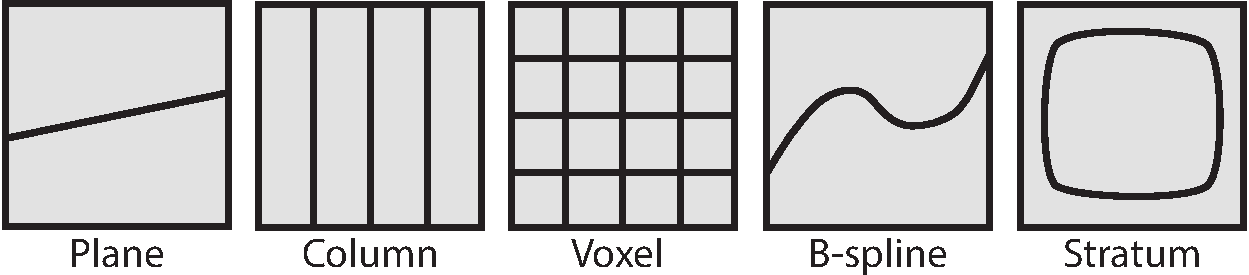
\includegraphics[width=0.7\linewidth]{figure/geometryNodes}
\caption{2D representations  of the \emph{geometry nodes} used in \emph{reducer trees}.}
\label{fig:geometryNodes}
\end{figure}

\paragraph{Material Nodes:} The \emph{leaf nodes} of the \emph{reducer tree} are the material parameterization nodes. These contain a material assignment function $\lambda\left(x\right)$ that maps spatial coordinates to materials. \emph{Material nodes} can assign a void material to regions of the volume. Hence, surface displacements and material assignments can be treated in a unified fashion.
While \emph{material node} can be extended to implement arbitrary material assignment functions
(such as functionally graded materials and lattice structures),
all the following results require only a single type of \emph{material node}, \emph{layered node}, which assigns $k$ material layers of varying thickness to a geometry partition.
As a special case, a constant material for a region can be implemented as a \emph{layered node} with a single layer.

\emph{Geometry nodes} and \emph{material nodes} can be connected into a tree structure that describes a material assignment function throughout the input geometry. 
The essential property of this data structure is that it naturally adapts to the input geometry. This key feature allows it to be reused for different shapes.
\autoref{fig:red1} shows two examples of \emph{reducer trees} and the resulting geometric distributions of materials.
The tree on the left can be used to produce objects with caustics effects.
The input shape is first divided into columns. Next, each column is sliced by a plane.
By assigning materials to lower parts of the columns, the microfacet surface is created.
On the right, I show a tree for producing objects with subsurface scattering properties.
The input shape is first divided using a \emph{stratum node}. Then, the outer layer is sliced into columns, which create a texture once materials are assigned. The inner part of the object obtains a material with given subsurface scattering properties.

Since the tree describes a nested set of partitions, it can efficiently perform material queries by passing a query point through the tree until it arrives at a parameterization node. 
Note that the \emph{reducer tree} does not inherently enforce material continuity between disjoint regions of the object; however, for material assignment problems, this is neither required nor desired. 

\begin{figure}[h]
\centering
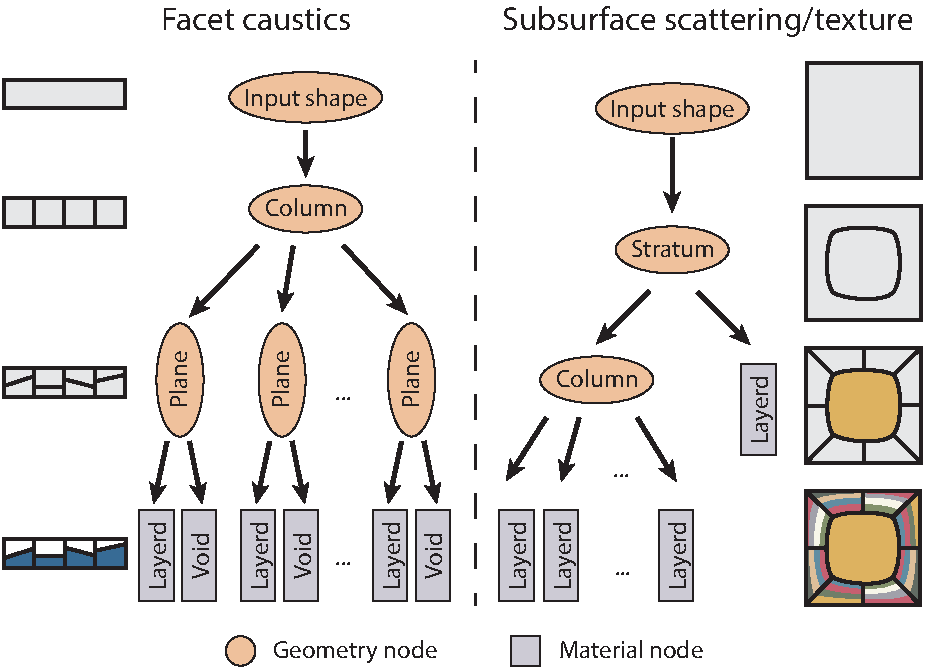
\includegraphics[width=0.7\linewidth]{figure/redNetworkNew.pdf}
\caption{Two examples of \emph{reducer trees}. Left: A tree for caustics effect.
Right: a tree for subsurface scattering properties.
}
\label{fig:red1}
\end{figure}

\section{Tuners and Tuning the Reducer Tree}
I define \emph{tuners} as an abstract interface between a \emph{reducer node} and an optimization algorithm. 
A \emph{reducer node} has parameters that control its space partitioning and material composition,
e.g., \emph{stratum node} has a parameter which determines its thickness,
\emph{column node} has parameters that control the width of columns.
A \emph{tuner} is responsible for tuning these parameters to achieve a specified goal.
A \emph{tuner} is comprised of an optimization scheme, an error metric, a simulator and a goal (\autoref{fig:tuner0}). 
In order to create an optimal material assignment, \emph{tuner nodes} must be attached to the \emph{reducer tree}.
The developer links each \emph{tuner} to a \emph{reducer node} in the \emph{reducer tree}.
Each \emph{tuner} then traverses the \emph{reducer subtree} (rooted at this \emph{reducer node})
and constructs a parameter list by querying each visited \emph{reducer node}.
The developer can label parameters as fixed or free. \emph{Tuner nodes} contain specific optimization routines
(e.g., a quadratic program solver).
The \emph{tuner node} then uses this routine to optimize its associated free parameters.
During execution, additional information (e.g., parameters, errors, etc.) from neighboring Tuner Nodes
can be obtained via the \emph{tuner network} (Section~\ref{sec:TunerNetwork}).
Tuner execution can be scheduled (again by the programmer) allowing both serial and parallel processing.

\begin{figure}[h]
\centering
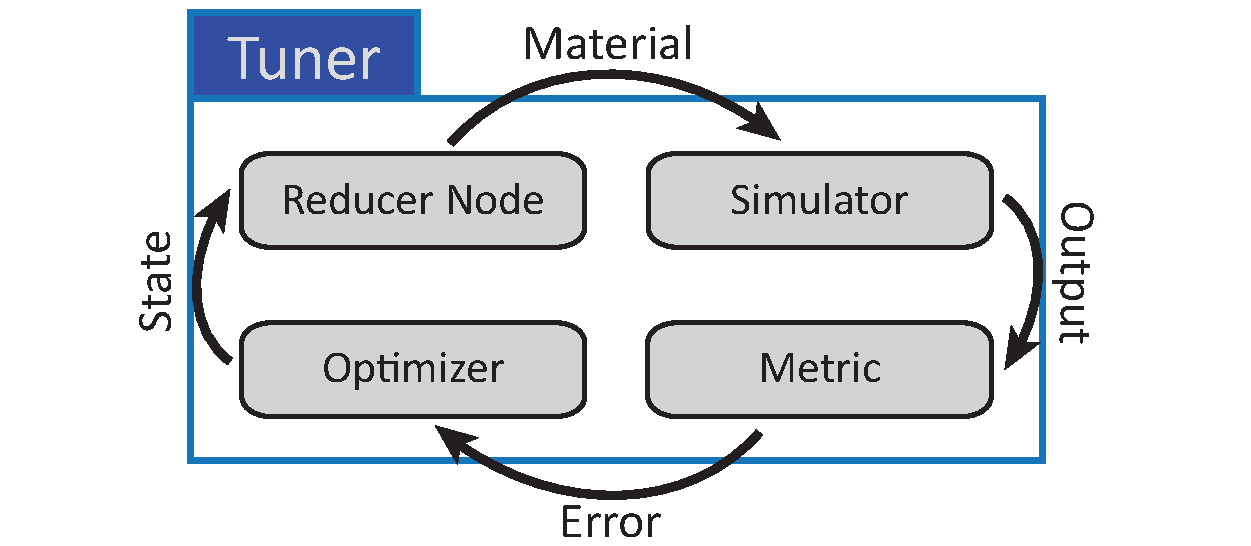
\includegraphics[width=0.6\linewidth]{figure/tuner2.pdf}
\caption{A diagram of the \emph{tuner} workflow. Arrows indicate flow and type of information passed between the individual \emph{tuner} components.}
\label{fig:tuner0}
\end{figure}

\autoref{fig:tunerCon} shows a simple example in which two \emph{tuners} are attached to sibling nodes in a \emph{reducer tree}. The first \emph{tuner} is responsible for \emph{layered} and \emph{void material nodes }while the second is responsible for several \emph{layered material nodes}.  

\begin{figure}[h]
\centering
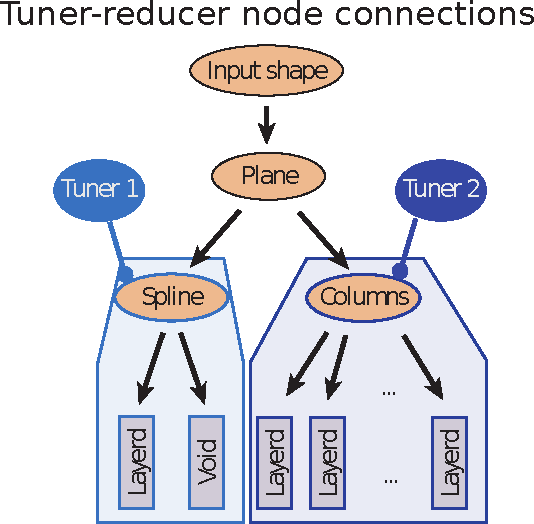
\includegraphics[scale=0.7]{figure/tunerCon.pdf}
\caption{ 
  Two \emph{tuners} attached to a \emph{reducer tree}. Each \emph{tuner} is responsible for tuning the nodes in its attached subtree (denoted by shapes with similarly colored outlines).}
\label{fig:tunerCon}
\end{figure}

\section{Tuner Network}
\label{sec:TunerNetwork}
For many fabrication problems, \emph{tuners} should not act in isolation. For instance, an optimal material assignment at a given point depends on the material assignment in the neighborhood. Tuning the free parameters without taking into account this dependency usually yields suboptimal results. Therefore, I allow the \emph{tuners} to share information according to a user-specified graph structure. This allows my framework to interface with a wide range of existing graph-based optimization and inference algorithms. For example, Figure~\ref{fig:tunerNet} shows one of the \emph{tuner networks}.

\begin{figure}[h]
\centering
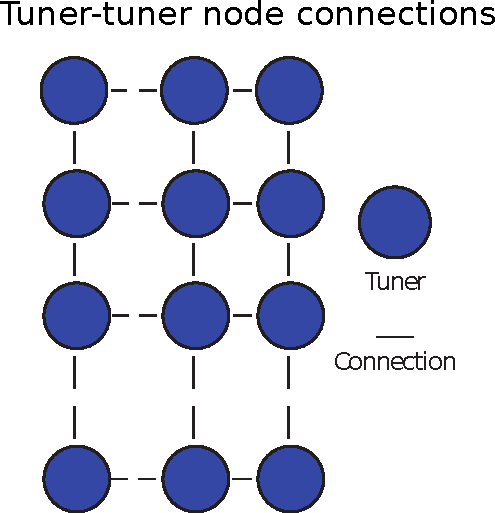
\includegraphics[scale=0.6]{figure/tunerNet.pdf}
\caption{ 
	One example of \emph{tuner network} that is used in experiments.}
\label{fig:tunerNet}
\end{figure}

In this network, each node is connected to its four neighbors.
In the following chapters, \emph{tuners} enclosed in dashed boxes are connected in this form.
\emph{Tuner networks} do not always exhibit this regular connectivity.
For instance, \emph{tuners} can be completely unconnected (\autoref{fig:tunerCon}) or be organized into groups which feature intra- but not inter-group connections.


\chapter{Process Configuration}
\label{sec:config}
In this section I show each step of process configuration. At the same time I describe my implementation of the 
\emph{reducer tree} and \emph{tuner network} data structures.

\section{Defining the Reducer Tree}
A \emph{reducer tree} can be constructed expediently using existing \emph{geometry} and \emph{material node} types.
\emph{Reducer trees} are not restricted to use only existing node types.
New node types can be added by extending the \verb|ReducerNode| class (see Figure~\ref{fig:node}).
In particular, implementing a new \emph{geometry node} type requires providing the function \verb|getOutputIndex|.
This function takes, as input, a 3D position and returns the \verb|id| of its child (Geometry or Material)
that contains this 3D point.
This function also computes a local coordinate for this child node.
Performing computations in local coordinates allows us to abstract away the geometry of a given object.
Implementing a new \verb|MaterialNode| type requires specifying the \verb|getMaterial| function
which takes a 3D point and returns the material at this point in the local geometry coordinate system.
Both types of nodes have an \verb|evaluate| function which is responsible for updating their internal states.
This function is used by the \emph{tuner network} to modify the internal state of the nodes.
As an example, we show a \emph{reducer tree} for performing texture mapping (see Figure~\ref{fig:red1}).
We also provide the corresponding pseudo-code (see Algorithm~\ref{alg:ReducerTree}).

\begin{figure}[h]
\centering
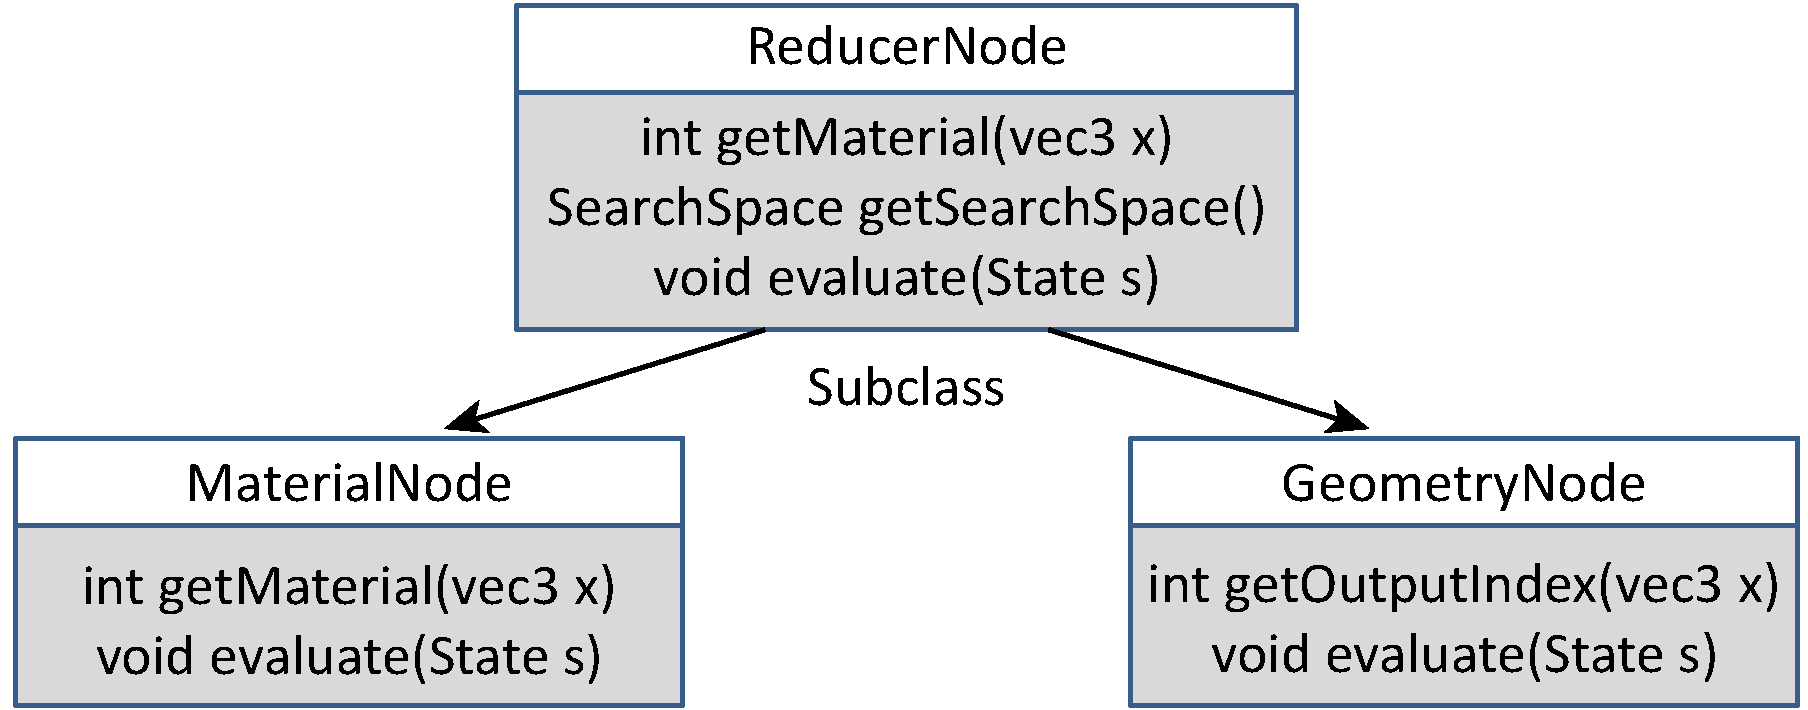
\includegraphics[width=0.6\linewidth]{figure/node.pdf}
\caption{Abstract interface for Node and its two subclasses.}
\label{fig:node}
\end{figure}

\begin{algorithm}
\caption{Constructing a \emph{reducer tree} for texturing}
\label{alg:ReducerTree}
\begin{lstlisting}[mathescape=true]
1. Create a root node $\mathbf{R}$ from inputMesh 
2. Subdivide $\mathbf{R}$ into outer layer $\mathbf{O}$ and inner volume $\mathbf{V}$ (Stratum Node) 
3. Subdivide $\mathbf{O}$ into set of columns $\mathbf{C}$ (Column Node) 
4. For each column $\mathbf{c}$ in $\mathbf{C}$ 
5.   Subdivide $\mathbf{c}$ into two layers (Layer Node) 
6. End 
\end{lstlisting}
\end{algorithm}

\section{Defining a \emph{Tuner}}
Recall that a \emph{tuner} consists of four components: a simulation, an error metric, an optimizer and a goal (\autoref{fig:tuner0}). Certain combinations of goal, metric and simulator are not compatible (i.e., a deformation simulator is not compatible with an error metric that compares images). Our API checks and prevents such incompatible combinations of components.  The optimization algorithm can request the error value for a given state using a callback function \verb|getError()| which is defined by the \emph{tuner}. Additional callback functions can be defined by the developer depending on the needs of the algorithm. For example, the branch and bound algorithm requires a custom  function to compute error bounds for a given state.

\section{Binding \emph{Tuners}}

\emph{Tuners} are assigned to nodes in the \emph{reducer tree} using the \verb|setNode| function. Once assigned, a \emph{tuner} can optimize the parameters of its associated subtree. \emph{Reducer nodes} provide a \verb|getSearchSpace| function which returns all free variables in the node subtree. In order to make \emph{tuners} as flexible as possible we provide a \verb|Parameter| class. Parameters can be either discrete or continuous, they can have associated bounds, and they can be marked as free or fixed.

\section{Establishing the \emph{Tuner Network}}

The \emph{tuner network} is an undirected graph that describes connections between \emph{tuners}.
\emph{Tuner nodes} store a list of their neighbors.
Only neighboring \emph{tuners} are allowed to exchange information.
In our current implementation, this is accomplished using a shared memory array.
As an example, we show how to construct and initialize a \emph{tuner network} for a simple optimization scheme --
a Simulated Annealing algorithm~\cite{Van:1987} (see Algorithm~\ref{alg:TunerNetwork}).
The \emph{tuner network} also requires a schedule that specifies in what order individual \emph{tuners} should be executed.
This schedule is specified by the developer. Once the \emph{tuner network} is constructed,
the process configuration phase is complete.
We obtain a compiled executable that computes desired material assignment from an input specification.
\begin{algorithm}
\caption{Connecting and executing the \emph{tuner network}}
\label{alg:TunerNetwork}
\begin{lstlisting}[mathescape=true]
1.  for each Tuner $\mathbf{T}_i$ attached to a plane
2.    for each Tuner $\mathbf{T}_j$ adjacent to $\mathbf{T}_i$
3.      add $\mathbf{T}_j$ to $\mathbf{T}_i$'s list of neighbors
4.    end
5.  end
6.  iterate N times
7.  for each Tuner $\mathbf{T}_i$
8.    set temperature for $\mathbf{T}_i$'s optimizer
9.    run $\mathbf{T}_i$
10. end
\end{lstlisting}
\end{algorithm} 
\section{Process Use}
\label{sec:use}
The compiled program, which executes the \emph{tuner network}, takes five types of arguments: the input geometry, the goal, the simulation configuration, a set of materials and the target 3D printer specification. 
After the \emph{tuner network} is executed, the parameters of the \emph{reducer nodes} in the \emph{reducer tree} are set. It is then straightforward to compute the material assignment at arbitrary resolution. Since, a typical multi-material 3D printer requires a volumetric model with per voxel material assignment, we can simply iterate over all voxels in the volume. We obtain the material assignment by evaluating (\verb|getMaterial|) of the \emph{reducer tree} root at the center of each voxel location. This representation can be easily converted to a printer specific format for output. For the Objet500 Connex printer used in this paper we extract material isosurfaces which are submitted to the printer as STL files. 
\chapter{Experiments}
\label{chap:results}
In order to evaluate capabilities of our system, I have implemented a number of existing translation processes.
Furthermore, the ease with which different algorithm components can be combined enables the creation of two new translation processes.
The first combination is an algorithm that can produce objects with desired refractive properties and an associated texture.
The second algorithm applies a desired texture to an object with prescribed deformation behavior.
All of these processes, both from prior work and new ones, should easily fit into our framework. I printed the objects using a Stratasys Object500 Connex  multi-material printer.
The following paragraphs provide a detailed description of how the individual algorithms can be designed with my system.
%All \emph{reducer trees} and the \emph{tuner networks} for producing these results are presented in 
%\autoref{fig:ReducerTreesAdditional}.

\section{Spatially-varying Albedo}
I have designed a Spec2Fab translator that allows 3D printing of textured models (Figure~\ref{fig:textured}).
The \emph{reducer trees} and the \emph{tuner networks} for producing these results are presented in 
\autoref{fig:treeTexture}.
Being able to apply precisely specified spatially-varying albedo values to printed models is a crucial capability.
However, no standard processes have been designed for this task so far.
The input to the texturing algorithm is a shape and its desired albedo texture.
Since the texture is only affected by materials close to the surface,
I use a \emph{stratum node} to divide the input shape into a thin shell and an inner volume.
I then divide the outer layer into columns.
The set of printable colors is expanded by stacking translucent materials using the \verb|LayeredMaterial| Node.
The number of layers is fixed to the number of print materials.
The reduced parameters are the thickness values of each material layer.
For each column, the \emph{tuner}'s optimizer looks up the proper stacking that produces the closest albedo value.
Due to printer resolution, the range of albedo values that can be achieved is quantized.
I therefore implement an error diffusion algorithm by connecting neighboring \emph{tuners}.
In this simple algorithm, the simulation is a table lookup using measured albedo value corresponding to different base materials.

\begin{figure*}[t]
\centering
\includegraphics[width=0.95\linewidth]{figure/texture.pdf}
\caption {The reducer-tuner model enables creating objects of arbitrary shapes with embedded textures.}
\label{fig:textured}
\end{figure*}

\begin{figure*}[t]
\centering
\includegraphics*[scale=0.7]{figure/treeTexture.pdf}
\caption{\emph{Reducer tree} for texture.}
\label{fig:treeTexture}
\end{figure*}

\section{Heterogeneous Subsurface Scattering}
I have replicated the subsurface scattering process of Ha\v{s}an et al.~\shortcite{Hasan:2010:PRO} using a tree
shown in Figure~\ref{fig:treeSubs}. A 3D printed chessboard is shown in Figure~\ref{fig:sub}.
The input to this algorithm is a 3D mesh along with subsurface-scattering profiles defined
at a set of surface points.
We use the same \emph{reducer tree} as in the texture example thereby simplifying the process configuration phase.
Since the \emph{reducer tree} adapts to the input geometry, I can apply the same marble material to arbitrary
meshes such as the dome shown in Figure~\ref{fig:dome}.
The only difference is that I allow each column to have four layers of varying thickness and material.
I use a branch and bound optimization algorithm which has been modified to handle continuous parameters by allowing discrete increments.
I implement a bound estimate callback function specific to this problem.
Each column is optimized independently using the algorithm. 
The simulation computes a scattering profile for a given stacking
and the error metric compares the simulated and goal profiles using squared error.
\begin{figure}[h]
\centering
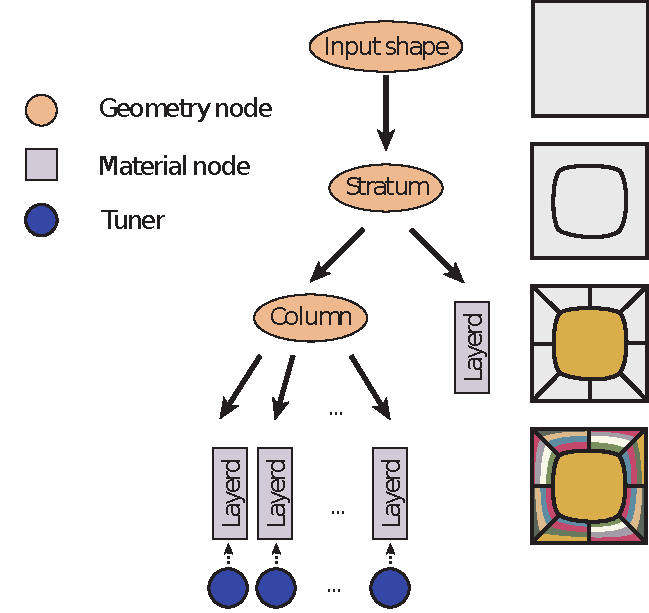
\includegraphics[scale=0.7]{figure/treeSubs.pdf}
\caption{
	\emph{Reducer tree} for heterogeneous subsurface scattering effect.}
\label{fig:treeSubs}
\end{figure}

\begin{figure}[h]
\centering
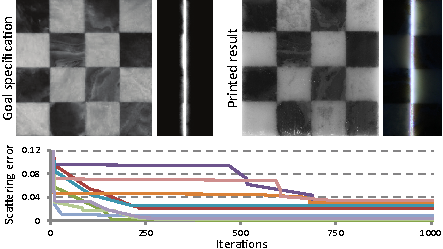
\includegraphics[width=0.65\linewidth]{figure/fig_chess.pdf}
\caption{
	A marble chessboard with prescribed subsurface scattering properties produced by Ha\v{s}an et al.~\shortcite{Hasan:2010:PRO}.
	The insets show the samples under thin line illumination, and the graph shows the convergence of tuners for 10 out of 100 scattering profiles used in the example. The error is measured by square distance between two profiles, each containing 400 coefficients.}
\label{fig:sub}
\end{figure}

\begin{figure}[h]
\centering
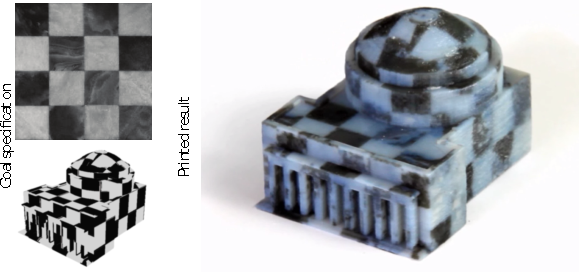
\includegraphics[width=0.75\linewidth]{figure/dome.pdf}
\caption{
	A marble dome produced by the subsurface scattering \emph{reducer tree}.}
\label{fig:dome}
\end{figure}

\section{Goal-based Caustics}
I have configured two different processes for computing goal-based caustics.
While they define exactly the same goal, they have very different \emph{reducer trees} and \emph{tuner networks}.
The first process is based on the work of Papas et al.~\shortcite{Marios:2011}.
It computes a set of micro-lenses which produce the desired caustic image as shown in Figure~\ref{fig:facet}.
The image is pre-processed into a set of Gaussian distributions.
Each distribution is matched with a microlens.
The optimization applies simulated annealing to permute the location of these micro-lenses
in order to construct a smooth surface.
The micro-lenses are represented using \emph{plane nodes}.
The complete reducer tree is shown in Figure~\ref{fig:treeFacet}.
In the \emph{tuner network}, each \emph{tuner} is connected to its four neighbors.
During the execution of an individual \emph{tuner},
the optimization algorithm makes a randomized decision
about whether or not to swap its micro-lens with one of its neighbors based on smoothness of the surface.
The \emph{tuners} are executed many times until a user-specified convergence criterion is met. 

\begin{figure}[h]
\centering
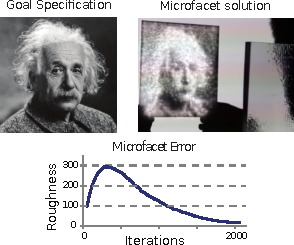
\includegraphics[width=0.65\textwidth]{figure/facet.pdf}
\caption {3D printed lens arrays that produce a caustic image of Einstein.
The algorithm is proposed by Papas et al.~\shortcite{Marios:2011}.
Below we show convergence plots for the microfacet optimizations.
The portrait is available from the United States Library of Congress's Prints and Photographs division,
now in the public domain.
}
\label{fig:facet}
\end{figure}

\begin{figure}[h]
\centering
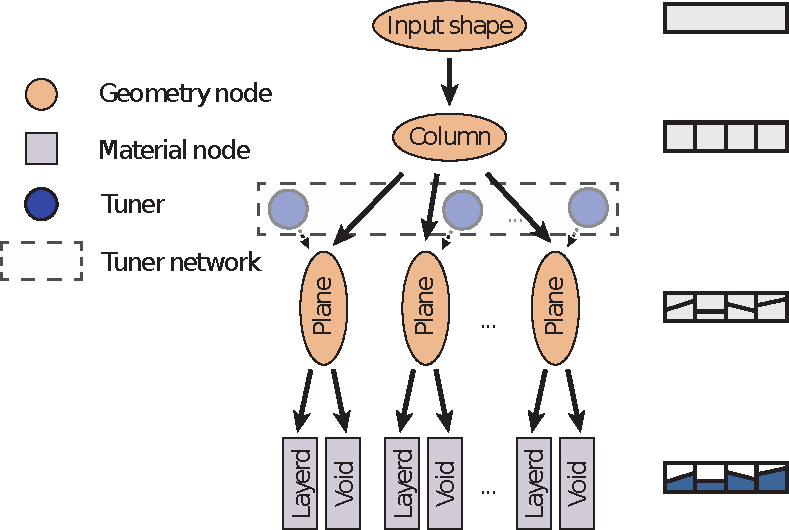
\includegraphics[scale=0.7]{figure/treeFacet.pdf}
\caption {\emph{Reducer tree} for facet caustics.
}
\label{fig:treeFacet}
\end{figure}

The second process is based on the work of Finckh et al.~\shortcite{Finckh:2010} (Figure~\ref{fig:spline}).
I use a \emph{B-spline node} to represent a smooth surface (Figure~\ref{fig:treeSpline}).
This is in contrast to the potentially discontinuous surface in the method above.
The reduced parameters are the height of each spline control point.
I implement a simple caustics simulator for height fields.
The simulated image is compared to the goal image using mean squared error.

\begin{figure}[h]
\centering
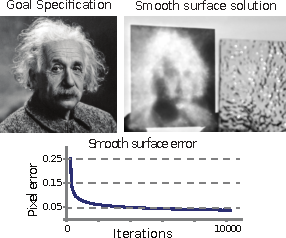
\includegraphics[width=0.65\textwidth]{figure/spline.pdf}
\caption {A smooth surface that produces a caustic image of Einstein.
The algorithm is proposed by Finckh et al.~\shortcite{Finckh:2010}.
Below we show convergence plots for the smooth surface optimization.
}
\label{fig:spline}
\end{figure}

\begin{figure}[h]
\centering
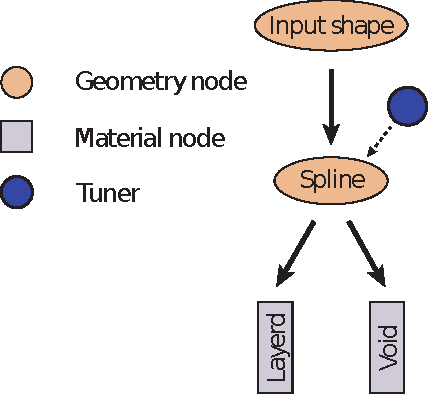
\includegraphics[scale=0.7]{figure/treeSpline.pdf}
\caption {\emph{Reducer tree} for smooth caustics.
}
\label{fig:treeSpline}
\end{figure}

\section{Elastic Behavior}
In the spirit of Bickel et al.~\shortcite{Bickel:2009},
I have implemented an algorithm to compute material distribution based on a desired force-displacement response.
The input to this algorithm is a mesh, a simulation configuration, and a desired shape.
Simulation configuration includes vertex constraints and forces applied to the mesh.
For this example, I use a co-rotational finite element method (FEM) simulation
with linearly elastic materials to estimate the objects deformation.
For the \emph{reducer tree} (Figure~\ref{fig:treeDeform},
I use a voxel partition to divide the object into a low-resolution grid.
I assign a single material to each grid cell.
The FEM simulator queries the \emph{reducer tree} for material assignments at arbitrary spatial locations.
I use the same branch and bound algorithm as in our subsurface-scattering process
but with a different bound computation callback function.
I use the mean squared distance between the simulated and the desired shapes as the error metric.
I have designed a simple experiment to validate this process
in which I set the goal of our optimization to be a given deformed state (\autoref{fig:book}).
\begin{figure}[h]
\centering
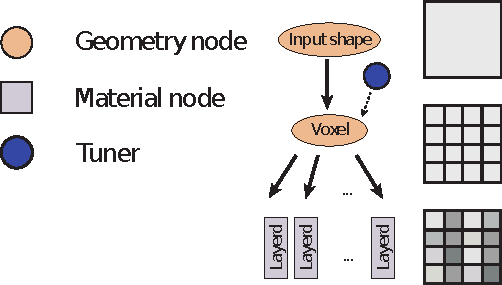
\includegraphics[scale=0.7]{figure/treeDeform.pdf}
\caption {\emph{Reducer tree} for elastic behavior.
}
\label{fig:treeDeform}
\end{figure}

\begin{figure}[h]
\centering
\includegraphics[width=0.65\linewidth]{figure/fig_sub.pdf}
\caption {A 3D printed book with prescribed deformation behavior under load.
The plot shows the error (in meters) as a function of iteration number of our branch and bound based \emph{tuner}.
The blue line shows the smallest error seen so far while the red line the \emph{tuner}'s progress exploring material subtrees~\protect\cite{Bickel:2009}.}
\label{fig:book}
\end{figure}

\section{Combining Deformable Object and Spatially-varying Albedo}
The first of my new translation processes combines spatially-varying albedo and elastic deformation properties
(Figure~\ref{fig:globe}).
This is a very useful combination since when modeling objects we would like to specify both their appearance and ``feel''.
In this process, the input shape is divided into a thin shell and an inner volume
(Figure~\ref{fig:treeTexDef}).
I optimize for the deformation behavior and the texture independently due to the limitations of our current FEM simulator.
As the outer shell is very thin, it has negligible influence on overall object deformation.
\begin{figure}[h]
\centering
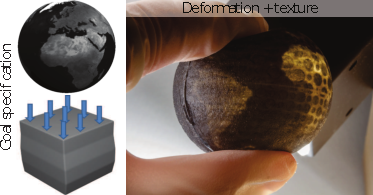
\includegraphics[width=0.7\textwidth]{figure/globe.pdf}
\caption {A miniature of Earth with prescribed deformation behavior.}
\label{fig:globe}
\end{figure}
\begin{figure}[h]
\centering
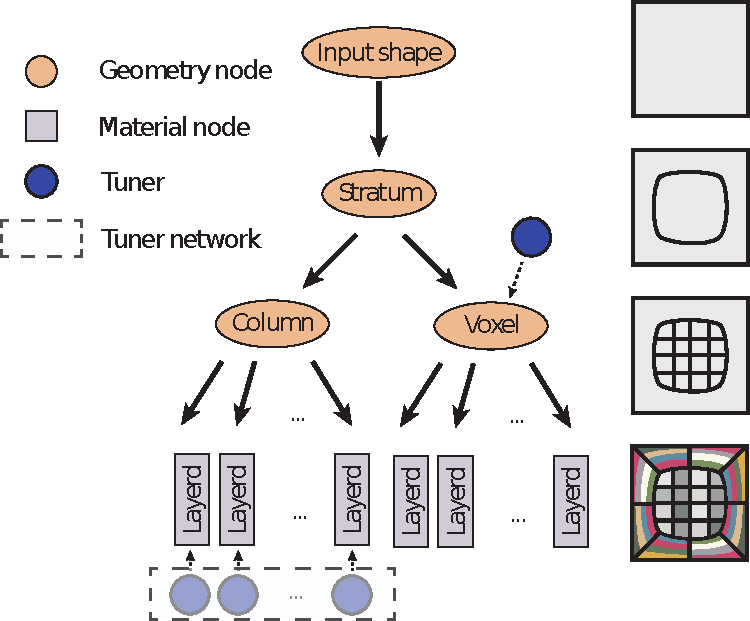
\includegraphics[scale=0.7]{figure/treeTexDef.pdf}
\caption {\emph{Reducer tree} for combining texture and elastic behavior.
}
\label{fig:treeTexDef}
\end{figure}

\section{Combining Caustics and Spatially-varying Albedo}
My second new combined translation process incorporates both smooth caustics and texture mapping
(Figure~\ref{fig:cake}).
More specifically, I compute a transparent slab with a texture image that, when illuminated, casts a prescribed caustic image.
The input slab is split into two pieces using a \emph{plane node} as shown in Figure~\ref{fig:treeTexSpline}.
The top piece is tuned to produce an input image. The material in the top piece is then fixed. The bottom piece is then tuned to produce a caustics image.
\begin{figure}[h]
\centering
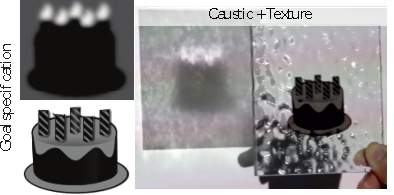
\includegraphics[width=0.7\textwidth]{figure/cake.pdf}
\caption {A textured smooth surface producing a designed caustics image under proper illumination.}
\label{fig:cake}
\end{figure}

\begin{figure}[h]
\centering
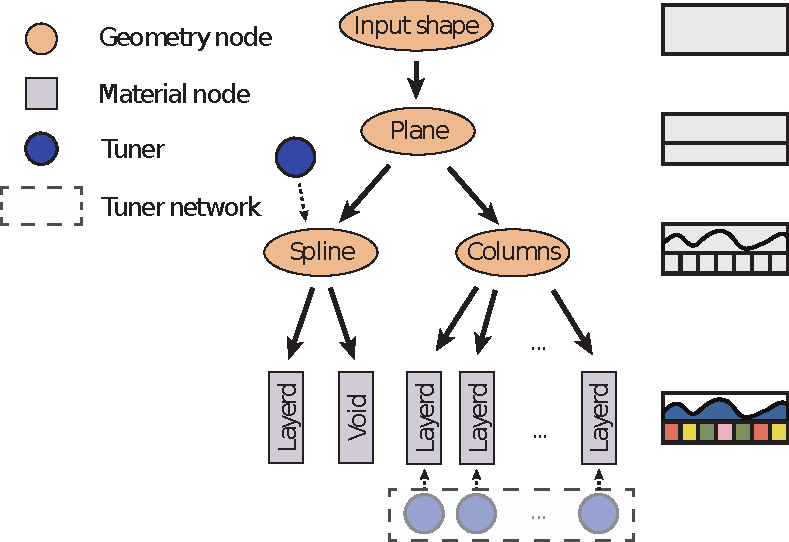
\includegraphics[scale=0.7]{figure/treeTexSpline.pdf}
\caption {\emph{Reducer tree} for combining texture and smooth caustics.
}
\label{fig:treeTexSpline}
\end{figure}

\chapter{Discussion}
Through my series of experiments, The \emph{reducer tree} and \emph{tuner network}
have allowed me to reuse a large number of software components.
In the extreme case, I arrive at my subsurface scattering algorithm
by trivially adapting the same \emph{reducer tree} for texture mapping objects.
The power of component reuse is further elucidated by the presence of \emph{column nodes} in most examples
and by the reuse of optimization schemes (such as branch and bound) in multiple algorithms.
The \emph{reducer tree} and \emph{tuner network} make these similarities easy to observe and exploit.
The only component whose reusability was not demonstrated in this proposal is simulation.
In this work, I have aimed to fabricate objects with a wide range of physical properties
and this necessitates the use of a wide range of simulation algorithms.
Finally, once a whole process is configured, it is independent of input geometry and goal parameters.
For example, I have run the spatially-varying albedo process with different geometries and input textures.

The \emph{reducer-tuner model} is ideally suited for multi-material printing
capable of producing objects with a wide range of different properties.
In order to showcase these strengths, I have fabricated my examples for an Objet500 Connex --
a phase change inkjet printer that uses photopolymers with a wide range of optical and mechanical properties.
Even though only two materials can be used and mixed within a single object,
my framework has been proven to be very useful. 
As the number of materials that can be printed simultaneously will grow,
I expect the methodology presented here to increase in utility.
For other types of 3D printing technologies, Spec2Fab framework has a reduced use. In the case of 3D printing using a single, rigid material (e.g., fused filament fabrication or Stereolithography) the framework can be used to tune geometry of objects. For plaster-based 3D printers that produce full-color 3D prints, Spec2Fab framework can be employed to compute proper texturing of objects.
\chapter{Conclusion}
In this research I have taken the first step towards solving an open problem in computational fabrication -- 
creating a general translation process that transforms user-defined model specifications into printer and material-specific representations.
My process relies on two data structures to make this general translation process expressive and computationally tractable: a \emph{reducer tree} and a \emph{tuner network}.
I have shown how existing instances of this translation can be expressed and combined within my system.
I believe that my API and its reference implementation will simplify and encourage development of new translation processes.

My system offers many exciting opportunities for future work.
First, it would be extremely useful to implement many additional simulators in order to allow computing a variety of other properties, e.g., structural soundness, stability, material cost, and printing time.
These simulators could be employed to expand the range of possible user-defined specifications.
Similarly, only relatively simple error metrics have been proposed within the tuning process.
The development of more sophisticated and, in particular, perceptually-driven material metrics remains a relatively unexplored research area.
Finally, it would be very beneficial to couple my API with a visual interface to further simplify the task of translator construction.
It is not obvious what the best visual interface for specifying functional or physical properties of these objects is and more research in this area is necessary.


%%%%%%%%%%%%%%
%% Back Matter
%%%%%%%%%%%%%%

% appendixes
\appendix
%\include{appendix1} % appendix1.tex should be in the same directory in this case
%\include{appendix2} % appendix2.tex should be in the same directory in this case

% bibliography
\cleardoublepage
\phantomsection
\addcontentsline{toc}{chapter}{Bibliography}
%\bibliographystyle{plain}
\bibliographystyle{plainnat}
\bibliography{paper} % use with BibTeX (bibliography.bib should be in the same directory in this case)

% index (uncomment the lines below if you want an index)
%\newpage
%\mbox{}
%\newpage
%\addcontentsline{toc}{chapter}{Index}
%\printindex

\end{document}
